% Exam Template for UMTYMP and Math Department courses
%
% Using Philip Hirschhorn's exam.cls: http://www-math.mit.edu/~psh/#ExamCls
%
% run pdflatex on a finished exam at least three times to do the grading table on front page.
%
%%%%%%%%%%%%%%%%%%%%%%%%%%%%%%%%%%%%%%%%%%%%%%%%%%%%%%%%%%%%%%%%%%%%%%%%%%%%%%%%%%%%%%%%%%%%%%

% These lines can probably stay unchanged, although you can remove the last
% two packages if you're not making pictures with tikz.
\documentclass[11pt,fleqn]{exam}
\RequirePackage{amssymb, amsfonts, amsmath,amsthm, mathtools, latexsym, verbatim, xspace, setspace,enumitem}
\RequirePackage{tikz, pgflibraryplotmarks}

% By default LaTeX uses large margins.  This doesn't work well on exams; problems
% end up in the "middle" of the page, reducing the amount of space for students
% to work on them.
\usepackage[margin=1in]{geometry}


% Here's where you edit the Class, Exam, Date, etc.
\newcommand{\class}{Math 1271 - Lectures 010 and 030 }
\newcommand{\term}{Fall 2017}
\newcommand{\examnum}{Midterm 2 - A}
\newcommand{\examdate}{11/09/17}
\newcommand{\timelimit}{50 Minutes}
\DeclarePairedDelimiter\abs{\lvert}{\rvert}%
% For an exam, single spacing is most appropriate
\singlespacing
% \onehalfspacing
% \doublespacing

% For an exam, we generally want to turn off paragraph indentation
\parindent 0ex
\def\changemargin#1#2{\list{}{\rightmargin#2\leftmargin#1}\item[]}
\let\endchangemargin=\endlist 
%%\usepackage{pgfplots}
%%\pgfplotsset{my style/.append style={axis x line=middle, axis y line=
%		middle, xlabel={$x$}, ylabel={$y$}, axis equal,width=\textwidth }}
%	\pgfplotsset{every x tick label/.append style={font=\small, yshift=0.5ex}}
%	\pgfplotsset{every y tick label/.append style={font=\small, xshift=0.5ex}}
	\renewcommand{\d}[1]{\ensuremath{\operatorname{d}\!{#1}}}
	\newcommand{\pydx}[2]{\frac{\partial #1}{\newcommand\partial #2}}
	\newcommand{\dydx}[2]{\frac{\d #1}{\d #2}}
	\newcommand{\ddx}[1]{\frac{\d{}}{\d{#1}}}
	\newcommand{\evat}[3]{\left. #1\right|_{#2}^{#3}}
	\newcommand{\restr}[2]{\evat{#1}{#2}{}}
\begin{document} 

% These commands set up the running header on the top of the exam pages
\pagestyle{head}
\firstpageheader{}{}{}
\runningheader{\class}{\examnum\ - Page \thepage\ of \numpages}{\examdate}
\runningheadrule

\begin{flushright}
\begin{tabular}{p{2.8in} r l}
\textbf{\class} & \textbf{Name (Print):} & \makebox[2in]{\hrulefill}\\
\textbf{\term} &&\\
\textbf{\examnum} &&\\
\textbf{\examdate} &&\\
\textbf{Time Limit: \timelimit} & Section & \makebox[2in]{\hrulefill}
\end{tabular}\\
\end{flushright}
\rule[1ex]{\textwidth}{.1pt}

You may \textit{not} use your books, notes, graphing calculator, phones or any other internet devices on this exam. Please show all work clearly and legibly.\\

%You are \textbf{required} to justify your answers rigorously on each problem on this quiz. Supporting evidence and/or informal justification may be redeemed for partial credit.\\
\hspace*{12cm}\begin{minipage}[t]{2.3in}
\vspace{0pt}
%\cellwidth{3em}
\gradetablestretch{2}
\vqword{Problem}
\addpoints % required here by exam.cls, even though questions haven't started yet.	
\gradetable[v]%[pages]  % Use [pages] to have grading table by page instead of question

\end{minipage}
%\newpage % End of cover page

%%%%%%%%%%%%%%%%%%%%%%%%%%%%%%%%%%%%%%%%%%%%%%%%%%%%%%%%%%%%%%%%%%%%%%%%%%%%%%%%%%%%%
%
% See http://www-math.mit.edu/~psh/#ExamCls for full documentation, but the questions
% below give an idea of how to write questions [with parts] and have the points
% tracked automatically on the cover page.
%
%
%%%%%%%%%%%%%%%%%%%%%%%%%%%%%%%%%%%%%%%%%%%%%%%%%%%%%%%%%%%%%%%%%%%%%%%%%%%%%%%%%%%%%


\begin{questions}

% Basic question
%\vspace*{-130pt}
\addpoints
%\begin{changemargin}{0pt}{137.4803pt} Find the real numbers within the interval $I$ at which $f$ is \emph{not} continuous. State whether $f$ is continuous from the right, the left, or neither.
%\begin{parts}
%\part[1] $\displaystyle{f(x)=\frac{1}{x^2+4x-21}}$\hfill $I=(-\infty,\infty)$\vskip1.5mm
%\part[1] $\displaystyle{f(x)=\frac{\sin{\frac{x}{2}}}{\cos{2x}}}$\hfill $I=[-\pi,\pi]$\vskip1.5mm
%\part[1] $\displaystyle{f(x)=\begin{cases}2^x&x\leq 3\\-3x+17&3<x\leq 4\\\frac{1}{\sqrt{x-3}}&x>4
%	\end{cases}}$\hfill $I=(-3,8)$
%\end{parts}
%\end{changemargin}
\newpage
\question[15] Consider the equation $y=\sqrt{x-2}$


\begin{parts}
\part Compute $\Delta y$ and $\d y$ at $x_0=3$ and $\d x =\Delta x=0.02$.
\part Use the previous part to compute an approximation to the number $\sqrt{1.02}$. \end{parts}

\newpage
\addpoints
\question[15] A water tank has the shape of an inverted circular cone with base-radius $R=3$m and height $H=9$m. If water is being pumped into the tank at a rate of 3 m${}^3/$min find:
%\begin{changemargin}{0pt}{137.4803pt}
\begin{parts}
\part the rate at which the water level is rising when the water is 6m deep.
\part the rate at which the radius of the water level is increasing when the water is 6m deep.
\end{parts}

\emph{Hint:} The volume $V$ of a cone with radius $r$ and height $h$ is $V=\frac{1}{3}\pi r^2h$.\begin{figure}[h!]
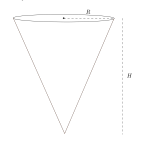
\includegraphics[scale=.6]{cone}
\end{figure}
%\end{changemargin}
\addpoints\newpage
\question[20]\begin{parts}
	\part State the definitions of critical and inflection numbers (or points).\vspace{1.5in}
	\part State the first and second derivative tests \vspace{1.5in}
	\part Consider the function $f(x)=\ln(x^2+4)$.%\newline
	\begin{enumerate}[label=(\roman*)]
		\item Find the intervals of increase and decrease for $f(x)$.
		\item Find the critical points of $f(x)$ and identify any local minima or maxima.
		\item Find the intervals of concavity.
		\item Find the inflection points of $f$. 
	\end{enumerate}
\end{parts}
\addpoints\newpage
\question[15] If 200 cm${}^2$ of material is available to make a closed box with a square base, find the largest possible volume.\addpoints\newpage

\question[20] Compute the value of the following limits:
\begin{parts}
	\part \[\lim_{x\to \infty}x^2e^{-x^2}\]
	\vspace{3.5in}
	\part \[\lim_{x\to \infty}x^{1/x}\]
\end{parts}
\addpoints\newpage
\question[15] Find $f(t)$ where $$f''(t)=\sqrt{t}-\sin(t),\;f(0)=1,\; f'(0)=-1$$

\end{questions}
\end{document}